%%***********************************************
%% 		Setups
%%***********************************************
\documentclass[12pt, letterpaper, titlepage]{article}
%	\setlength{\columnsep}{31pt}		% space b/w columns;

% margins
\usepackage[top=.5in, bottom=1.2in, left=.7in, right=.7in]{geometry}

% title
\title{\Huge CSE 105: \\ Computation
	   \\[-1em] \rule{.8\textwidth}{1pt}
}
\author{\LARGE{\it by} Jy}
\date{}
%\thanks{}

%***********************************************
% 		Graphs
%***********************************************

%% space of caption and the context;
%	\setlength{\abovecaptionskip}{10pt}
%	\setlength{\belowcaptionskip}{15pt}
%\usepackage{subfigure}
\usepackage{graphicx}
	\graphicspath{{pics/}}

%% figures with text wrapped around;
%\usepackage{wrapfig}
%\usepackage{picins}

\usepackage{tikz}
%	\usetikzlibrary{arrows}
%%\usepackage{tkz-euclide}
%\usepackage{pgfplots}
%	\tikzset{
%	myvec/.style={blue, line width = .5pt, -stealth'},
%	every node/.style={black},
%	box/.style={rectangle, rounded corners=5pt,
%			minimum width=30pt, minimum height=15pt,
%			inner sep=5pt,
%			draw=silver, fill=lightpurple},
%	}

% trees
\usepackage{tikz-qtree}
% \usepackage{pst-tree}

%% set wallpaper
%\usepackage{wallpaper}
%	\CenterWallPaper{1}{}

%% Include movies
%\usepackage{media9}

%% use colors
\usepackage{xcolor}
	\definecolor{lightblue}{RGB}{39, 104, 192}
	\definecolor{silver}{RGB}{200,191,231}
	\definecolor{lightpurple}{RGB}{200,200,240}

%%***********************************************
%% 		Tables
%%***********************************************

% linestrech in arrays/tables
\renewcommand{\arraystretch}{1.2}

%% tables w/ wrapped lines;
%\usepackage{tabularx}
%	\newcommand{\ahsize}[1]{ \setlength{\hsize}{#1\hsize} }
%	\newcommand{\bhsize}[1]{ \setlength{\hsize}{#1} }

%% sideways
\usepackage{rotating}

%% makecell
%\usepackage{makecell}
%	\makegapedcells
%	\setcellgapes{6pt}

%% color for tables;
%\usepackage{colortbl}
%% toprule, midrule & bottomrule;
%\usepackage{booktabs}
\usepackage{array} %解决前置命令问题;
	\newcommand{\PreserveBackslash}[1]{\let\temp=\\#1\let\\=\temp}
	\newcolumntype{C}[1]{>{\PreserveBackslash\centering}p{#1}}
	\newcolumntype{R}[1]{>{\PreserveBackslash\raggedleft}p{#1}}
	\newcolumntype{L}[1]{>{\PreserveBackslash\raggedright}p{#1}}
	\newcolumntype{M}[1]{>{$}#1<{$}}

%% multirow;
\usepackage{multirow}

%% long table + tabularx;
%\usepackage{ltxtable, filecontents}

%%***********************************************
%% 		Coding
%%***********************************************

%	\usepackage{listings}
%		\lstset{
%			language=C++,
%			breaklines=true,				%自动换行;
%			extendedchars=false,			%这一条命令可以解决代码跨页时,章节标题,页眉等汉字不显示的问题;
%			numbers=left,
%			numberstyle=\scriptsize,
%			stepnumber=2, 				%行标跳过数;
%			numbersep=1.5em, 				%行标与代码框距离;
%			tabsize=4,
%			basicstyle=\footnotesize\ttfamily,
%			stringstyle=\color{lightblue},
%			keywordstyle=\color{blue!80},
%			commentstyle=\color{red!70!green!70!blue!90},
%			frame=shadowbox,
%%			showspaces=false,
%			showstringspaces=false,
%			showtabs=false,
%			rulesepcolor=\color{red!20!green!20!blue!20},
%			backgroundcolor=\color{red!10!green!3!blue!10},
%			escapeinside=``,
%			xleftmargin=8em,
%			xrightmargin=5em,
%			framexleftmargin=2pt,
%			framexrightmargin=2pt,
%			aboveskip=1em
%		}
%		\renewcommand{\lstlistingname}{CODE}

%***********************************************
% 		Fonts
%***********************************************

%% English;
\usepackage{fontspec}
	\setmainfont[Mapping=tex-text]{Times New Roman}
	\setsansfont[Mapping=tex-text]{Calibri}
	\setmonofont{Courier New}
%	\newfontfamily\rh{Lucida Handwriting}	% rh for Round Handing
%	\newfontfamily\sc{John Handy LET}	% sc for script
%	\newfontfamily\hw{Bradley Hand ITC}	% hw for HandWritting
%% Chinese;
%\usepackage[CJKchecksingle, CJKnumber]{xeCJK}
%	\setCJKmainfont[BoldFont = {STXingkai}, ItalicFont = {STFangsong}]{Microsoft YaHei}
%	\setCJKsansfont{}
%	\setCJKmonofont{KaiTi}
%	\punctstyle{hangmobanjiao}
%\newcommand{\CJKdash}{\rule[3.5pt]{9pt}{.77pt} \hspace{-1.5mm} \rule[3.5pt]{9pt}{.77pt} }

%%***********************************************
%% 		Looking
%%***********************************************

%% links
\usepackage[bookmarksnumbered, pdfencoding=auto, pdfborder=1, breaklinks,
			colorlinks, linkcolor=lightblue, urlcolor=blue]{hyperref}
	\hypersetup{
		unicode=false,			% non-Latin characters in Acrobat’s bookmarks
		pdftoolbar=true,		% show Acrobat toolbar?
		pdfmenubar=true,		% show Acrobat menu?
		pdftitle={},			% title
		pdfauthor={Jinyao Yuan},% author
		pdfsubject={},			% subject of the document
		pdfcreator={Jinyao Yuan},	% creator of the document
		pdfproducer={Jinyao Yuan},	% producter of the document
		citecolor=green,		% color of links to bibliography
		filecolor=magenta,		% color of file links
	}

	%% page style
	%%---------------------------------------------------------------------------
	\usepackage{fancyhdr}
	\pagestyle{fancy}
	\lhead{}
	\chead{}
	\rhead{}
	\renewcommand{\headrulewidth}{0pt}
	\renewcommand{\footrulewidth}{0pt}
	\lfoot{}
	\cfoot{}
	\rfoot{\thepage}

%% paragraphs
%%---------------------------------------------------------------------------
\usepackage{setspace}
	\onehalfspacing
%	\doublespacing
	\setlength{\parindent}{2em}
	\addtolength{\parskip}{3pt}
	\usepackage{indentfirst}

%% floats
%%---------------------------------------------------------------------------
% \renewcommand{\textfraction}{0.15}
% \renewcommand{\topfraction}{0.85}
% \renewcommand{\bottomfraction}{0.65}
\renewcommand{\floatpagefraction}{0.70}

\usepackage[section]{placeins}
% \usepackage[below]{placeins}
\usepackage{caption}

%% underline
%%---------------------------------------------------------------------------
\usepackage{ulem}
%\usepackage{CJKfntef}

%% emphasis
%%---------------------------------------------------------------------------
% \DeclareTextFontCommand{\emshape}{\itshape}
\def\emshape{\itshape}
\makeatletter
\DeclareRobustCommand{\em}{%
    \@nomath\em \if b\expandafter\@car\f@series\@nil \normalfont
    \else \emshape \fi
}
\makeatother
\DeclareTextFontCommand{\emph}{\em}

%% convert terms into Chinese;
%%---------------------------------------------------------------------------
%\renewcommand{\contentsname}{\hfill 目~录 \hfill}
%\renewcommand{\listfigurename}{图目录}
%\renewcommand{\listtablename}{表目录}
%\renewcommand{\thepart}{\CJKnumber{\arabic{part}}}
%\renewcommand{\partname}{第\CJKnumber{\thepart}章}
%\renewcommand{\thesection}{\CJKnumber{\arabic{section}}}
%\newcommand{\sectionname}{\thesection 节}
%\renewcommand{\figurename}{图}
%\renewcommand{\figureautorefname}{图}
%\renewcommand{\tablename}{表}
%\renewcommand{\tableautorefname}{表}
%\renewcommand {\thefootnote}{\arabic{footnote}}
%\renewcommand{\footnoteautorefname}{脚注}
%\renewcommand{\abstractname}{摘 \quad 要}
%\renewcommand{\appendixname}{附录{\thechapter}}
%\renewcommand{\appendixautorefname}{附录}
%\renewcommand{\bibname}{参考文献}
%\renewcommand{\indexname}{索引}

%% make own style of section titles;
%%---------------------------------------------------------------------------
\usepackage{titlesec}
%	\titleformat{\part}{\center\Huge \bf}{\thepart}{1em}{}
%	\titleformat{\section}{\large \bf}{\thesection}{1em}{}
	\titleformat{\part}[frame]{\normalfont}
		{\small \enspace UNIT \thepart \enspace}{6pt}
		{\LARGE\bf\filcenter}
	\titlespacing*{\part}{1pc}{*4}{*3}[1pc]
	\newcommand{\mypart}{\FloatBarrier\part}

%% make own style of table of contents;
%%---------------------------------------------------------------------------
%\usepackage{titletoc}
%\titlecontents{part}[0em]{\addvspace{10pt}\filright\bf\large}
%		{\def\numberline##1{\thecontentslabel\quad\ignorespaces}}
%		{}{\titlerule*[8pt]{.}\contentspage}
%\titlecontents{section}[1em]{\addvspace{10pt}\filright\bf\large}
%		{\def\numberline##1{\thecontentslabel\quad\ignorespaces}}
%		{}{\titlerule*[8pt]{.}\contentspage}
%\titlecontents{subsection}[2em]{\addvspace{5pt}\filright\bf}
%		{\def\numberline##1{\thecontentslabel\quad\ignorespaces}}
%		{}{\titlerule*[8pt]{.} \contentspage}

%***********************************************
% 		Utilities
%***********************************************

%% in-para enum, item, descript;
%%---------------------------------------------------------------------------
\usepackage{paralist}

%% lettrine;
%%---------------------------------------------------------------------------
%\usepackage{lettrine}
%	\newcommand{\mylettrine}[1]{\lettrine[lines=2,lraise=0,nindent=0em]{#1\hspace{1mm}}{}}

%% Math;
%%---------------------------------------------------------------------------
\usepackage{amsmath, amsfonts, amssymb, amsthm}
\usepackage{venndiagram}
%\usepackage{extarrows} 	% special arrows like \xlongequal;
%\input{longdiv.tex}	% divisions;
%\usepackage{dcolumn}	% vertical calculation w/ tabular;
\usepackage{cancel}	% strike out numbers

%% Theorems;
%%---------------------------------------------------------------------------
\newtheoremstyle{mystyle}
	{2em}	% spaceabove
	{2em}	% spacebelow
	{\it}	% bodyfont
	{0em}	% indent
	{\bf}	% headfont
	{}   	% headpunctuation
	{1em}	% headspace
	{%
		\thmname{#1} \thmnumber{#2} \thmnote{#3}.
	}   	% headspecify
\theoremstyle{mystyle}

\newtheorem{definition}{Definition}[section]
\newtheorem{theorem}{Theorem}[section]

%% symbols
%%---------------------------------------------------------------------------
\newcommand{\phteq}{ \phantom{{}={}} }
\renewcommand{\(}{ \left(  }
\renewcommand{\)}{ \right) }
\newcommand{\nth}{\ensuremath{^\text{th}}\xspace}
\newcommand{\st}{\ensuremath{^\text{st}}\xspace}
\newcommand{\nd}{\ensuremath{^\text{nd}}\xspace}
\newcommand{\rd}{\ensuremath{^\text{rd}}\xspace}
\newcommand{\dd}{{ \, \mathrm{d} }}
\newcommand{\abs}[1]{{ \left\lvert #1 \right\rvert }}

\newcommand{\set}[1]{{ \left\{\,#1\,\right\} }}
\newcommand{\lst}[1]{{ \left(\,#1\,\right) }}

%\newcommand{\dne}{ \mathrm{DNE} }	% Does Not Exist;
%\newcommand{\defeq}{ \xlongequal{\mathrm{DEF}} }	% equal by definition;
%\newcommand{\sqr}{ \ensuremath{^2} } % squared;
% \newcommand{\cels}{{ \ensuremath{^\circ \mathrm{C}} }}
%\newcommand{\fahr}{{ \ensuremath{^\circ \mathrm{F}} }}
\newcommand{\Conf}{{ \mathrm{Conf} }}
\newcommand{\true}{{ \text{\upshape True} }}
\newcommand{\false}{{ \text{\upshape False} }}

\newcommand{\DFA}{{ M = \lst{Q, \Sigma, \delta, s, F} }}
\newcommand{\NFA}{{ N = \lst{Q, \Sigma, \delta, s, F} }}
\newcommand{\reverse}{{ \mathrm{rev} }}
\newcommand{\combination}{{ \mathrm{C} }}
\newcommand{\permutation}{{ \mathrm{P} }}
\newcommand{\variance}[1]{{ \mathrm{Var}(#1) }}
\newcommand{\stirling}{{ \mathrm{S} }}
\newcommand{\powerset}{{ \mathcal{P} }}
\newcommand{\Degree}{{ \mathbb{Deg} }}
\newcommand{\degree}{{ \mathbb{deg} }}

%% visiblespace
\renewcommand\textvisiblespace[1][.5em]{%
	\makebox[#1]{%
		\kern.07em
		\vrule height.3ex
		\hrulefill
		\vrule height.3ex
		\kern.07em
	}
}

%% fillable forms
%%---------------------------------------------------------------------------
%\newcommand{\fform}[2]{
%#1 \vbox{\hbox{\TextField[name=#1,width=#2,borderwidth=0]{\null}}\kern0pt\hrule}
%}

%% Margin notes;
%%---------------------------------------------------------------------------
\usepackage{marginnote}
\marginparsep 2em
\marginparwidth 2.5in

% fancy boxes like \fbox,\shadowbox,\doublebox,\ovalbox, \Ovalbox。
\usepackage{fancybox}

%%***********************************************
%%	Self-defined environments
%%***********************************************

\usepackage{float} % used to define float environments

%% list point
%%---------------------------------------------------------------------------
%\newcommand{\lspnt}[1]{&\textrm{#1}}
%\newenvironment{pntlist} {
%	$
%	\left\{
%	\begin{aligned}
%}{
%	\end{aligned}
%	\right.
%	$
%}

%% centered graph
%%---------------------------------------------------------------------------
\newcommand{\centgraph}[2][.7\linewidth]{
	\begin{center}
		\includegraphics[width=#1]{#2}
	\end{center}
}

%% questions & solutions
%%---------------------------------------------------------------------------
%\input{environment.question/quest.tex}

% shadowpage
%---------------------------------------------------------------------------
\newenvironment{shadowpage}%
{
	\begin{Sbox} \begin{minipage}
	}{
	\end{minipage} \end{Sbox}
	\setlength{\fboxsep}{10pt}
	\shadowbox{\TheSbox}
}%

% examples
%---------------------------------------------------------------------------

%\floatstyle{plaintop}
%\newfloat{exp}{htb}{log}[subsection]
%\floatname{exp}{Example}
\DeclareCaptionType[%
	placement=htbp,
	within=section,
	fileext=loe
]{myExample}[Example][List of Examples]
\newenvironment{example}[1][~]%
{%
	\begin{myExample}
		\hfill
		\begin{Sbox}
			\begin{minipage}{.8\linewidth}
				\footnotesize
				\vspace{-.5em} \caption{#1} ~ \\[-2em]
				\rule{\linewidth}{.3pt}
				\par
				\setlength{\parindent}{2em}
				\addtolength{\parskip}{3pt}
			}{%
			\end{minipage}
		\end{Sbox}
		\setlength{\fboxsep}{10pt}
		\shadowbox{\TheSbox}
	\end{myExample}
}%

%\newenvironment{example}%
%{
%	\par\noindent
%	\hfill
%	\begin{Sbox}
%	\begin{minipage}{.8\linewidth}
%	\footnotesize
%	{\bf Example} \\[-1em]
%	\rule{\linewidth}{.5pt}
%	\par
%	\setlength{\parindent}{2em}
%}{
%	\end{minipage}
%	\end{Sbox}
%	\setlength{\fboxsep}{10pt}
%	\fbox{\TheSbox}
%	\par
%}%



%***********************************************
% 		START
%***********************************************
\begin{document}

\maketitle
\pagenumbering{roman}
\tableofcontents\clearpage
\pagenumbering{arabic}


\section{Deterministic Finite Automaton (DFA)}
% ==================================================

A machine consists of different states drawn in circles with names. Often a state drawn as
a double circle is an ``acceptive state,'' and a plain circle indicates a ``rejective
state.'' A machine receives a string consisted of `1's and `0's as input and the states
change as the machine reads through input digits. An arrow is used to indicate which state
is to start with. See \autoref{exa:a_DFA} for detailed information.

\subsection{Expressions of DFA's}
% --------------------------------------------------

\begin{example}[A DFA]
    \label{exa:a_DFA}

    Let's first look at the DFA below which starts at state $A$.
    \centgraph{mp/dfa-0.pdf}

    If the string ``010110'' is input to the machine, will it result in true or false?
    Will the state be acceptive or rejective?
    \[
        \xrightarrow{010110}
        \fbox{M}
        \xrightarrow{1/0 \text{ (True / False, Accept / Reject)}}
    \]

    There are two arrows leaving state $A$: one with a label reading `1' which points to
    state $B$ and one reading `0' which goes back to state $A$ itself. That means, if an
    input digit reads `1,' the state changes to $B$, and if `0' the state stays in $A$.

    Now step through the procedure:
    \begin{compactenum}
    \item
        The machine starts off at state $A$ with input `0,' which, as explained above,
        changes the state to $A$ itself.
    \item
        Next, the second digit `1' is read so the state is changed to $B$.
    \item
        The next digit `0' makes state $B$ to switch to state $C$.
    \item
        Then state $C$ reads `1' so no state change occurs.
    \item
        The next digit is `1' again so the state remains still on $C$.
    \item
        Last, the digit `0' switches the state from $C$ to $B$.
    \end{compactenum}
    Thus the input string ``010110'' changes the machine to state $B$, which is an
    acceptive state.

\end{example}

\begin{definition}[DFA]
    \label{def:DFA}

    A DFA is a $5$-tuple
    \[ \DFA \]
    where
    \begin{compactdesc}
    \item[$Q$]      is a finite set,    for states
    \item[$\Sigma$] is a finite set,    for input alphabet
    \item[$s$]      $\in Q$,            for start states
    \item[$F$]      $\subseteq Q$,      for accepting states
    \item[$\delta$]
        $Q \times \Sigma \mapsto Q$,
        a function that specifies the transition between states
    \end{compactdesc}
\end{definition}

\begin{example}[Denoting machine in \autoref{exa:a_DFA}]

    According to definition \autoref{def:DFA}, 
    the machine in \autoref{exa:a_DFA} can be denoted by 
    \[ \DFA \]
    where
    \begin{compactitem}
    \item $Q        = \set{ A,B,C }$
    \item $\Sigma   = \set{ 0,1 }$
    \item $s        = \set{ A }$
    \item $F        = \set{ B,C }$
    \end{compactitem}
    And function $\delta$ can be described by the table below.
    \begin{center} \begin{tabular}{Mc Mc Mc}
        \hline
        \delta & 0 & 1  \\
        \hline
        A      & A & B  \\
        B      & C & A  \\
        C      & B & C  \\
        \hline
    \end{tabular} \end{center}

\end{example}

\begin{definition}[$f_M$]
    For any DFA $\DFA$,
    let 
    \[
        f_M : \Sigma^* \mapsto \set{ \true, \false }
    \]
    where $\Sigma^*$ is a set of strings over $\Sigma$.

    \[
        f_M(w)
        = \begin{cases}
            \true,   &\delta^*(s,w) \in F  \\
            \false,  &\text{else}
        \end{cases}
    \]
\end{definition}

\begin{definition}[$\delta^*$]
    \[
        \delta^* : Q \times \Sigma^* \mapsto Q
    \]
    which is an inductive function defined as
    \[
        \begin{cases}
            \delta^*(q, \varepsilon) = q \\
            \delta^*(q, aw) = \delta^*\( \delta(q,a), w \)
        \end{cases}
    \]
    where $varepsilon$ is an empty string and $q \in Q, a \in \Sigma, w \in \Sigma^*)$.
\end{definition}



\subsection{Configurations of DFAs}
% --------------------------------------------------

\begin{definition}[Configurations]
    \[
        \Conf = Q \times \Sigma^*
    \]
\end{definition}

\begin{definition}[Initial Configurations]
    The initial configuration of a machine $I_M(w) \in \Conf$
    \[
        I_M(w) = ( s,w )
    \]
\end{definition}

\begin{definition}[Final Configurations]
    The final configuration of a machine $H_M(w) \subseteq \Conf$
    \[
        H_M(w) = \set{ (q,u) \mid q \in Q, u = \varepsilon }
    \]
\end{definition}

\begin{definition}[Output]
    The output of a machine is a function that returns either ``$\true$'' or ``$\false$.''
    \[
        O_M \colon H_M \mapsto \set{ \true,\false }
    \]
    defined as
    \[
        O_M(q,\varepsilon)
        = \begin{cases}
            \true,   & q \in F  \\
            \false,  & \text{else}
        \end{cases}
    \]
\end{definition}

\begin{definition}[Transition Relations] %% ?
    $R_M \subseteq \Conf$

    \[
        R_M = \rightarrow_M
        = \{
            (q, aw) \rightarrow \( \delta(q,a),w\)
            \mid q \in Q, a \in \Sigma, w \in \Sigma^*
        \}
    \]
\end{definition}

\begin{example}[Configurations of machine in \autoref{exa:a_DFA}]
    With input ``10010'' write in mathematical language the configurations of machine in
    \autoref{exa:a_DFA}:
    \begin{align*}
        I_M (10010)
        =               (A, 10010)
        \rightarrow     (B, 0010)
        \rightarrow     (C, 010)
        \rightarrow     (B, 10)
        \rightarrow     (A, 0)
        \rightarrow     (A, \varepsilon)
        \in             H_M
    \end{align*}
    And thus the output
    \[
        O_F (A,\varepsilon) = \false
    \].

    The machine in fact will only accept integers that are \emph{not} multiples of 3.
\end{example}

\begin{definition}[]
    \[
        f'_n (w) = O_F (C_n)
    \]
\end{definition}

% \[
%     L(M) = \set{ w \in \Sigma^* \mid f_M(w) = \true }
%     L(M_1)  \Sigma^*
% \]



A subset of $\Sigma^*$ of a DFA that contains all inputs to which the output of the
machine is $\true$ is called the \emph{language} of the machine.

\begin{definition}[Regularity of Language]
    $ L \subseteq \Sigma^* $
    is regular if
    \[
        \exists {\text{\upshape DFA} M} \mid L(M) = L
    \]
\end{definition}

\begin{example}[]
    Given that
    $\varepsilon^* = \set{\varepsilon}$
    and
    $\Sigma^* = \set{\varepsilon,1,0,10,101,\cdots} = \set{0,1}^*$,
    which of the following languages are regular?
    \begin{compactitem}
%     \item
%         $L_1 = \set{ w \in \set{0,1}^* \mid w \text{ is not a multiple of } 3}$,
    \item
        $L_1 = \set{ w \in \set{0,1}^* \mid w \text{ is a power of } 2}$, and
    \item
        $L_2 = \set{ w \in \set{0,1}^* \mid w \text{ is a power of } 3}$.
    \end{compactitem}
    
    $L_1$ is regular while $L_2$ is not. A binary number that is a power of $2$ consists
    of only one $1$ and all other digits should be $0$s. A DFA that recognizes the
    language would be
    \centgraph{mp/dfa-1.pdf}

\end{example}

\begin{definition}[Operations on Languages] \ \\
    \begin{compactdesc}
    \item[Complement]
        $L^C = \set{w \in \Sigma^* \mid w \notin L}$
    \item[Union]
        $L_1 \cup L_2 = \set{w \in \Sigma^* \mid w \in L_1 \vee w \in L_2}$
    \item[Intersection]
        $L_1 \cap L_2 = \set{w \mid w \in L_1 \wedge \in L_2}$
    \item[Concatenation]
        $L_1 \cdot L_2 = \set{w_1 \cdot w_2 \mid w \in L_1, w_2 \in L_2}$
    \end{compactdesc}
\end{definition}

\begin{example}[If $L$ is regular, is $L^C$ also regular?]
    Yes.

    \begin{proof}[Proof of statement $\mathbb R$ is closed under complement.]
        Let $L \in \mathbb R,$
        prove $L^C \in \mathbb R:$

        By definition, 
        \[
            \exists \DFA \text{ s.t.\ } L(M) = L.
        \]

        Let $M' = \lst{Q,\Sigma,\delta,s,F^C},$

        then $L(M') = L(M)^C = L^C.$

        $L^C \in \mathbb R$ because $L^C = L(M').$
    \end{proof}
\end{example}

\begin{example}[$\forall L_1, L_2$ \\ 
    $
        L_1 \in \mathbb R \vee L_2 \in \mathbb R
        \implies L_1 \cup L_2 \in \mathbb R
    $]
        Yes, $\mathbb R$ is closed under union.
\end{example}



\section{Nondeterministic Finite Automaton (NFA)}
% ==================================================

\begin{example}[How many states do you need?]
    \[
        L = \set{ w \in \set{0,1}^* \mid \text{the $5$th digit of $w$ is $0$} }
    \]

    \centgraph{mp/dfa-2.pdf}

    What if the digits are counted from the right, i.e.\ the last 5th digit?

    \centgraph{mp/dfa-3.pdf}

\end{example}

\begin{definition}[NFA]
    An NFA is a $5$-tuple
    \[ \NFA \]
    where
    \begin{compactitem}
    \item $Q$ and $\Sigma$ are finite sets
    \item $s \in Q, F \subseteq Q$
    \item $\delta \colon
        Q \times \Sigma_\varepsilon
        \footnote{$\Sigma_\varepsilon = \Sigma \cup \set\varepsilon$}
        \mapsto \powerset(Q)$
    \end{compactitem}

\end{definition}


\begin{definition}[Configurations of NFA]
    \begin{align*}
        \Conf &= Q \times \Sigma^*
        \\
        I(w)  &= (s, w)
        \\
        H     &= Q \times \set\varepsilon
        \\
        O(q,\varepsilon) &=
                            \begin{cases}
                                \true,  & q \in F  \\
                                \false, & \text{else}
                            \end{cases}
        \\
        R &= \set{
            (q,aw) \mapsto (q',w) \mid
            \forall q \in Q, a \in \Sigma_\varepsilon, w \in \Sigma^*
        }
    \end{align*}
\end{definition}

\begin{definition}[Language of NFA]
    \[
        L(N) = \set{ w \mid \exists \text{accepting computation on input $w$} }
    \]
\end{definition}

\begin{theorem}
    \label{thm:NFA_to_DFA}
    \begin{align*}
        \forall \text{\upshape DFA} \NFA,  \\
        \exists \text{\upshape DFA} M = \lst{ Q',\Sigma,\delta',s',F' }
        \text{ s.t.\ }
        L(N) = L(M)
    \end{align*}
\end{theorem}

\begin{proof}[Proof of \autoref{thm:NFA_to_DFA}]
    \begin{align*}
        Q' &= \powerset(Q)  \\
        F' &= \set{ A \subseteq Q \mid A \cap F \not= \varnothing }  \\
        s' &= E(\set{s}) = \set{q \in Q \mid \exists s
                                                \xrightarrow\varepsilon q_1
                                                \xrightarrow\varepsilon q_2
                                                \xrightarrow\varepsilon q_3
                                                \cdots
                                                \xrightarrow\varepsilon q
        }  \\
        \delta'(A, a) &= E( \operatorname*\cup_{q \in A} \delta(q,a) )
    \end{align*}
\end{proof}


\section{Applications of Finite Automata}

A finite automaton can be applied to
\begin{compactitem}
\item defining models of computation,
\item testifying equivalence between models,
\item etc.
\end{compactitem}

\begin{definition}[Reverse]
    For a string,
    \[
        \reverse\big( \lst{a_1,a_2,\cdots, a_n} \big) = \lst{a_n, \cdots, a_2, a_1};
    \]
    For a language,
    \[
        \reverse(L) = \set{ \reverse(w) \mid w \in L }.
    \]
\end{definition}

It is easy to find that
\[
    \forall L \in \mathbb R, \reverse (L) \in \mathbb R.
\]

\begin{example}[$\mathbb R$ is closed under union]
    \label{exa:dem_R_closed_under_union}

    Recall \autoref{exa:R_closed_under_union}, with NFA it is much easier to proof the
    theorem now.

    \begin{proof}[Proof of \autoref{exa:R_closed_under_union}]
        Let $M_1, M_2$ be NFAs for $L_1$ and $L_2$,
        build an NFA for $L_1 \cup L_2$
        by simply adding a new initial state that transit to $s_1$ and $s_2$ with
        $\varepsilon$ arrows:
        \centgraph[3cm]{mp/nfa-4.pdf}
    \end{proof}
\end{example}

\begin{example}[$\mathbb R$ is closed under concatenation]
    \begin{proof}
        Let $M_1, M_2$ be NFAs for $L_1$ and $L_2$,
        build an NFA for $L_1 \cdot L_2$:
        \begin{compactenum}
        \item use a new initial state that transit to $s_1$ and $s_2$ with $\varepsilon$
            arrows as in \autoref{exa:dem_R_closed_under_union}; and
        \item change the final states in $M_1$ to regular states and connect them to $s_2$
            with $\varepsilon$ arrows.
        \end{compactenum}
        A rough graph that represents the above steps is
        \begin{center}
            \begin{minipage}{4cm}
                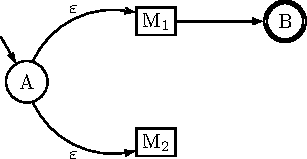
\includegraphics[width=\textwidth]{mp/nfa-5.pdf}
            \end{minipage}
            \; $\longrightarrow$ \;
            \begin{minipage}{4cm}
                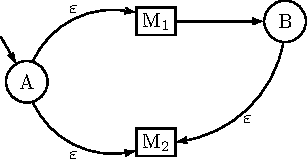
\includegraphics[width=\textwidth]{mp/nfa-6.pdf} 
            \end{minipage}
        \end{center}
        so
        \[
            L(M) = L(M_1) \cdot L(M_2) = \set{ wv \mid w \in L(M_1), v \in L(M_2) }.
        \]
    \end{proof}
\end{example}



% no Haskell on exams.

\section{Regular Expression}
% ==================================================

\subsection{Regular Language}
% --------------------------------------------------

We've learned that the class of regular languages is closed under
\begin{compactitem}
\item union,
    \footnote{
        $
        \text{ if } L_1, L_2 \in \mathbb R,
        \text{ then }
        L_1 \cup L_2 = \set{ w \mid w \in L_1 \lor w \in L_2 }
        \in \mathbb R
        .$
    }
\item intersection,
    \footnote{
        $
        \text{ if } L_1, L_2 \in \mathbb R,
        \text{ then }
        L_1 \cap L_2 = \set{ w \mid w \in L_1 \land w \in L_2 }
        \in \mathbb R
        .$
    }
\item concatenation, and
    \footnote{
        $
        \text{ if } L_1, L_2 \in \mathbb R,
        \text{ then }
        L_1 \cdot L_2 = \set{ w_1w_2 \mid w_1 \in L_1 \land w_2 \in L_2 }
        \in \mathbb R
        .$
    }
\item star.
    \footnote{
        $
        \text{ if } L \in \mathbb R,
        \text{ then }
        L^* = \set{ w_1w_2 \cdots w_n \mid w_1,w_2,\cdots,w_n \in L, n \ge 0 }
        \in \mathbb R
        .$
    }
\end{compactitem}

Many complex languages can be built using these operations; \autoref{exa:language_numbers}
is one practical example.

\begin{example}[Build a rather complex language]
    % any number with commas
    It is common we want to search for all numbers, say, in a file. The following set is a
    language that matches all numbers greater than $10$ and allowing appearance of commas.
    \[
        L =
        \set{1,\cdots,9} \cdot
        \( \set{0,1,\cdots,9}^* \cdot \set{,} \)^* \cdot
        \set{0,1,\cdots,9}
    \]

    Consider 
    \begin{align*}
        L_1 = \set{1,\cdots,9} \\
        L_2 = \set{0,1,\cdots,9}^* \cdot \set{,}  \\
        L_3 = \set{0,1,\cdots,9}  \\
    \end{align*}
    so 
    $L = L_1 \cdot L_2^* \cdot L_3$.

    What are $L_1$, $L_2$ and $L_3$?
    \begin{compactdesc}
    \item[$L_1$] is a set of all digits from $1$ to $9$;
    \item[$L_3$] is a set of all digits from $0$ to $9$;
    \item[$L_2$] is a little more complicated, it can also be written as $L_3^* \cdot
        \set{,}$, while $L_3^*$ matches a string of any number of elements in $L_3$, that
        is, a string made of all digits with unknown length. What $\cdot \set{,}$ does is
        it appends a comma to the end of this string. In all, $L_2$ is a number of digits
        with a comma at the end.
    \end{compactdesc}

    With that, the set $L_1 \cdot L_2^* \cdot L_3$ can be now (roughly) seen as:
    \[
        a digit \text{ and }
        a number of ( a number of digits \text{ and } a comma ) \text{ and }
        a digit
    \]
    Now, notice there is a leading digit and an ending one, why should one be in $L_1$ and
    the other $L_3$? Because matching from set $L_1$ rules out the numbers with leading
    $0$s ($L_1$ doesn't have $0$), and the rest of digits should allow $0$s. The middle
    portion ($L_2^*$) allows unknown number of strings from $L_2$ (even $0$) in between
    the first and last digit. In the case where the number of $L_2$ is $0$, which makes
    the input string also in set $L_1 \cdot L_3$, the input string is a two-digit number
    ($10$ to $99$).
\end{example}

\begin{example}[$\mathbb R$ closed under star]
    \begin{proof}
        use $\varepsilon$ transition from the final states to the initial states
        (including states transited directly from the initial state with an $\varepsilon$
        arrow) to prove that $\mathbb R$ is closed under star.
    \end{proof}
\end{example}

\subsection{Regular Expression}
% --------------------------------------------------

A regular expression (abbreviated regex or regexp) is a sequence of characters that forms
a search pattern, mainly for use in pattern matching with strings, or string matching,
i.e. "find and replace"-like operations.
(via \href{http://en.wikipedia.org/wiki/Regular_expression}{WikiPedia})

A regex $E$ has the following rules
\begin{align*}
    & E = a                   && L(a) = \set{a}                        \\
    & E = \varepsilon         && L(\varepsilon) = \set{\varepsilon}    \\
    & E = E_1 \cdot E_2       && L(E) = L(E_1) \cdot L(E_2)            \\
    & E = E_1 + E_2           && L(E) = L(E_1) + L(E_2)                \\
    & E = (E_1)^*             && L(E) = L\((E_1)^*\) = L(E_1)^*        \\
    & E = \varnothing         && L(\varnothing^*)
\end{align*}
In fact, the rule
\[
    L(\varepsilon) = \set{\varepsilon}
\]
can be replaced with 
\[
    L(\varnothing^*).
\]

\begin{theorem}[Equivalence of Regex and Regular Language]
    \[
        \forall L \in \mathbb R,
        \exists \text{ Regex } E \text{ s.t.\ } L(E) = L.
    \]
\end{theorem}

\subsection{GNFA}
% --------------------------------------------------

A generalized nondeterministic finite automaton (GNFA) is an NFA where
\begin{compactitem}
\item there are exactly one arrow entering and one leaving a state,
\item states can be transited using regexes ($\varnothing$ arrows, star arrows, etc.),
\item there are no arrows entering the initial state,
\item there is only one final state, and
\item there are no arrows leaving the final state.
\end{compactitem}

\begin{definition}[GNFA]
    A GNFA is defined as a $5$-tuple
    \[
        \lst{ Q,\Sigma,\delta,s,f }
    \]
    where
    \[
        \delta \colon
        (Q \backslash \set{f}) \times (Q \backslash \set{s})
        \mapsto
        \mathbb R(\Sigma)
    \]
\end{definition}

A GNFA, since it can use transitions with regexes, can help develop a regex of the
language of the GNFA by removing states one at a time until we have the form
\centgraph[3.5cm]{mp/gnfa-0}

The concept of regex finely relates to all automata we've learned so far:
\centgraph[3cm]{mp/relation_automata_regex-0}



\end{document}

